\documentclass[border=1mm]{standalone}
\usepackage{pgfplots}
\usepgfplotslibrary{groupplots}
\pgfplotsset{compat=1.17}
\usepackage{xcolor}
\usepackage{xstring}
\usepackage{tikz}



\definecolor{color1}{rgb}{0,0.4470,0.7410}
\definecolor{color2}{rgb}{0.8500,0.3250,0.0980}
\definecolor{color3}{rgb}{0.9290,0.6940,0.1250}
\definecolor{color4}{rgb}{0.4940,0.1840,0.5560}
\definecolor{color5}{rgb}{0.4660,0.6740,0.1880}


\begin{document}

\pgfplotsset{
compat=1.11,
legend image code/.code={
\draw[mark repeat=2,mark phase=2]
plot coordinates {
(0cm,0cm)
(0.3cm,0cm)        %% default is (0.3cm,0cm)
(0.6cm,0cm)         %% default is (0.6cm,0cm)
};%
}
}


\pgfdeclarelayer{background layer}
\pgfdeclarelayer{foreground layer}
\pgfsetlayers{background layer,main,foreground layer}

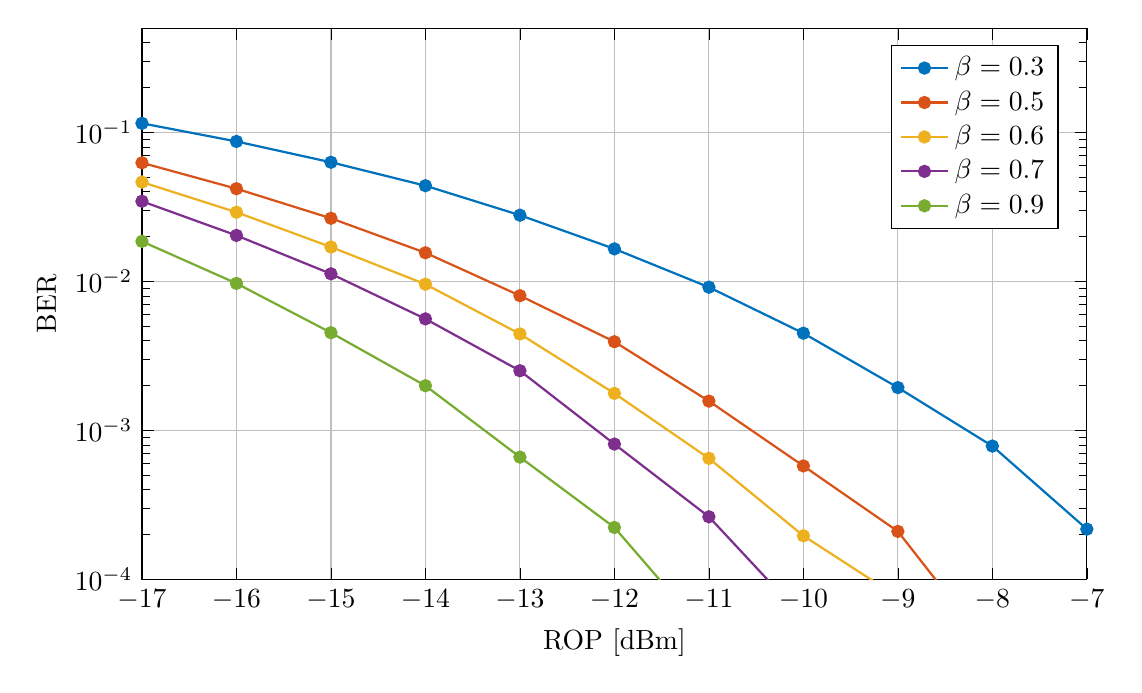
\begin{tikzpicture}[
]
\begin{semilogyaxis}[%
width=12cm,
height=7cm,
scale only axis,
every outer x axis line/.append style={black},
every x tick label/.append style={font=\color{black}},
every x tick/.append style={black},
xmin=-17,
xmax=-7,
xlabel={ROP [dBm]},
every outer y axis line/.append style={black},
every y tick label/.append style={font=\color{black}},
every y tick/.append style={black},
ymin=0.0001,
ymax=0.5,
ylabel={BER},
axis background/.style={fill=white},
xmajorgrids,
ymajorgrids,
%xtick={-33,-31,...,-5},
%ytick={0,0.25,...,2.25},
legend pos=north east
]
\addplot [thick,color1, mark=*] coordinates {(-17,0.1150125)(-16,0.086934375)(-15,0.063023125)(-14,0.043864375)(-13,0.02781125)(-12,0.0165325)(-11,0.00914)(-10,0.00448875)(-9,0.001938125)(-8,0.000785)(-7,0.0002175)};
\addlegendentry{$\beta=0.3$}

\addplot [thick,color2, mark=*] coordinates {(-17,0.062505625)(-16,0.041870625)(-15,0.0265175)(-14,0.01556375)(-13,0.008019375)(-12,0.00393625)(-11,0.0015725)(-10,0.0005775)(-9,0.00021)(-8,3.25e-05)(-7,8.75e-06)};
\addlegendentry{$\beta=0.5$}

\addplot [thick,color3, mark=*] coordinates {(-17,0.046374375)(-16,0.02912375)(-15,0.01701)(-14,0.009571875)(-13,0.004439375)(-12,0.00177125)(-11,0.000649375)(-10,0.00019625)(-9,7.625e-05)(-8,8.75e-06)(-7,0.0)};
\addlegendentry{$\beta=0.6$}

\addplot [thick,color4, mark=*] coordinates {(-17,0.034494375)(-16,0.020341875)(-15,0.011240625)(-14,0.005601875)(-13,0.00251375)(-12,0.000809375)(-11,0.000263125)(-10,5.5e-05)(-9,1.75e-05)(-8,0.0)(-7,0.0)};
\addlegendentry{$\beta=0.7$}

\addplot [thick,color5, mark=*] coordinates {(-17,0.0185525)(-16,0.009693125)(-15,0.00452625)(-14,0.001995)(-13,0.000661875)(-12,0.000223125)(-11,4.125e-05)(-10,1.375e-05)(-9,8.125e-06)(-8,0.0)(-7,0.0)};
\addlegendentry{$\beta=0.9$}



\end{semilogyaxis}

\end{tikzpicture}


\end{document}
























